\section{\texorpdfstring{Řešení úloh prohledáváním (DFS, BFS, uniform-cost, A${}^\ast$, heuristiky)}{Řešení úloh prohledáváním (DFS, BFS, uniform-cost, A*, heuristiky)}}

Mnoho úloh umělé inteligence lze zformulovat jako hledání \emph{posloupnosti akcí}, která agenta převede z~výchozího stavu do stavu cílového. Takový \emph{problémově orientovaný agent} pracuje s~\emph{atomickou} reprezentací stavů (stav je nedělitelný „černý box``), cíl popisuje množinou cílových stavů a~akce popisují přechody mezi stavy. Řešení se hledá \emph{prohledáváním}. Předpokládáme přitom prostředí \emph{plně pozorovatelné, diskrétní, statické a~deterministické}: agent zná svůj stav i~výsledek každé akce, takže může celou posloupnost naplánovat dopředu a~pak ji slepě provést.

\subsection{Formulace úlohy}

\begin{definice}[Dobře definovaná úloha]
Úloha prohledávání je dána čtveřicí:
\begin{itemize}
  \item \textbf{počáteční stav} $s_0$;
  \item \textbf{přechodový model} (a~množina akcí): pro stav $s$ je $A(s)$ množina použitelných akcí a~$\textsc{Result}(s,a)$ je stav po provedení akce $a$ ve stavu $s$;
  \item \textbf{test cílovosti}, který rozhodne, zda je daný stav cílový;
  \item \textbf{cena cesty}: nezáporná \emph{cena akce} (kroku) $c(s,a,s')$; cena cesty je součet cen jejích kroků.
\end{itemize}
\emph{Stavový prostor} (graf, jehož vrcholy jsou stavy a~hrany akce) je tím zadán \emph{implicitně} -- nevypisujeme ho celý, jen ho generujeme po krocích. \emph{Řešením} je posloupnost akcí z~$s_0$ do nějakého cílového stavu; \emph{optimální} řešení má nejmenší cenu cesty.
\end{definice}

\begin{intuice}
Klíčem k~rozumné formulaci je \emph{abstrakce}: ze stavu světa ponecháme jen to, co je pro úlohu podstatné. Abstrakce musí být \emph{platná} (každé abstraktní řešení lze rozvinout na řešení v~detailnějším světě) a~\emph{užitečná} (jednotlivé akce se provádějí snáz než původní úloha). Bez abstrakce by agenta reálný svět okamžitě zahltil.
\end{intuice}

\begin{priklad}[8-puzzle jako úloha prohledávání]
V~hlavolamu 8-puzzle je $3\times 3$ mřížka s~osmi očíslovanými kostkami a~jedním volným místem; tahem posuneme kostku na sousední volné místo. \textbf{Stav} = rozmístění kostek (a~volného místa); \textbf{počáteční stav} = zadané rozmístění; \textbf{akce} = posun volného místa nahoru/dolů/vlevo/vpravo (ekvivalentně posun sousední kostky), \textbf{cena} každého kroku $=1$; \textbf{test cílovosti} = shoda se zadaným cílovým rozmístěním. Stavový prostor má $9!/2 = 181\,440$ dosažitelných stavů (poloviny permutací jsou nedosažitelné kvůli paritě). Plné řešení této úlohy je níže (SZZ jaro 2024).
\end{priklad}

\subsection{Strom versus graf prohledávání}

Jádro každého prohledávacího algoritmu je stejné: udržujeme \emph{hranici} (frontier, otevřený seznam) ještě nerozvinutých uzlů, opakovaně z~ní podle nějaké \emph{strategie} vybereme uzel, \emph{rozvineme} ho (vygenerujeme jeho následníky a~přidáme je na hranici) a~končíme, jakmile narazíme na cílový uzel (nebo je hranice prázdná).

\begin{algo}[Obecné prohledávání (strom / graf)]
\ttfamily\small
GRAPH-SEARCH(úloha):\\
\hspace*{1.5em}frontier $\leftarrow$ \{ uzel s~počátečním stavem $s_0$ \}\\
\hspace*{1.5em}explored $\leftarrow$ $\emptyset$ \cmt{closed list; jen u~grafového prohledávání}\\
\hspace*{1.5em}\textbf{while} frontier $\neq \emptyset$:\\
\hspace*{3em}$n \leftarrow$ vyber uzel z~frontier \cmt{strategie: FIFO / LIFO / min $g$ / min $f$}\\
\hspace*{3em}\textbf{if} $n.\mathrm{stav}$ je cílový: \textbf{return} cesta k~$n$\\
\hspace*{3em}přidej $n.\mathrm{stav}$ do explored\\
\hspace*{3em}\textbf{for} každý následník $n'$ uzlu $n$:\\
\hspace*{4.5em}\textbf{if} $n'.\mathrm{stav} \notin$ explored (a~není už na frontier): přidej $n'$ na frontier
\end{algo}

\noindent\textbf{Stromové prohledávání} vynechá množinu \texttt{explored}: tatáž konfigurace se tak může objevit ve více uzlech a~algoritmus \emph{opakovaně rozvíjí} už navštívené stavy (prochází redundantní cesty). \textbf{Grafové prohledávání} si pomocí \texttt{explored} (closed list) pamatuje rozvinuté stavy a~každý stav rozvine \emph{nejvýš jednou}; strom prohledávání pak obsahuje každou konfiguraci nanejvýš jednou. Cenou za úsporu času je paměť na uložení \texttt{explored}. (Pseudokód výše testuje cílovost \emph{při výběru} uzlu z~hranice; u~BFS lze testovat už \emph{při generování} následníka, což je rychlejší, ale u~uniform-cost a~A${}^\ast$ by to vedlo k~neoptimálnímu řešení -- tam musí být test až při výběru.)

\begin{center}
\begin{tikzpicture}[scale=1.0]
% --- levá část: stavový graf s cyklem ---
\node[uzel] (A) at (0,2) {$A$};
\node[uzel] (B) at (-1,1) {$B$};
\node[uzel] (C) at (1,1) {$C$};
\node[uzel] (D) at (0,0) {$D$};
\draw[hrana] (A)--(B); \draw[hrana] (A)--(C);
\draw[hrana] (B)--(D); \draw[hrana] (C)--(D);
\node[font=\small] at (0,-0.8) {stavový graf};
% --- pravá část: strom prohledávání ---
\begin{scope}[xshift=5cm]
\node[uzel] (rA) at (0,2) {$A$};
\node[uzel] (rB) at (-1,1) {$B$};
\node[uzel] (rC) at (1,1) {$C$};
\node[uzel] (rD1) at (-1,0) {$D$};
\node[uzel] (rD2) at (1,0) {$D$};
\draw[sipp] (rA)--(rB); \draw[sipp] (rA)--(rC);
\draw[sipp] (rB)--(rD1); \draw[sipp] (rC)--(rD2);
\node[font=\small] at (0,-0.8) {strom (stromové prohl.)};
\end{scope}
\end{tikzpicture}
\obrpopis{Stav $D$ je dosažitelný dvěma cestami ($A\!-\!B\!-\!D$ a~$A\!-\!C\!-\!D$). \emph{Stromové} prohledávání proto $D$ rozvine \textbf{dvakrát} (pravý strom má dva uzly $D$); \emph{grafové} prohledávání drží closed list a~rozvine $D$ jen jednou. Redundance roste exponenciálně s~hloubkou, takže u~grafů (cykly, více cest) je grafové prohledávání zásadní.}
\end{center}

\subsection{Neinformované prohledávání}

\emph{Neinformované} (slepé) strategie nemají o~úloze žádnou informaci nad rámec její definice; liší se jen tím, který uzel z~hranice vyberou.

\begin{definice}[BFS, DFS, uniform-cost]
\begin{itemize}
  \item \textbf{Prohledávání do šířky} (BFS): hranice je fronta \emph{FIFO}, rozvíjí se vždy \emph{nejmělčí} nerozvinutý uzel.
  \item \textbf{Prohledávání do hloubky} (DFS): hranice je zásobník \emph{LIFO}, rozvíjí se vždy \emph{nejhlubší} nerozvinutý uzel.
  \item \textbf{Uniform-cost} (Dijkstra): rozvíjí se uzel s~\emph{nejnižší cenou cesty} $g(n)$; test cílovosti se provádí až při \emph{výběru} uzlu (ne při generování), jinak hrozí neoptimální řešení.
\end{itemize}
\end{definice}

\begin{intuice}
BFS je úplné (najde řešení, je-li větvení konečné) a~je \emph{optimální}, pokud cena roste nezáporně s~hloubkou (typicky jednotkové ceny). Platí za to ale pamětí: musí držet celou hranici, časová i~prostorová složitost je $O(b^{d})$ ($b$ = faktor větvení, $d$ = hloubka cíle). \emph{Paměť je u~BFS větší problém než čas.}

DFS sám o~sobě \emph{není} optimální a~ve stromovém prohledávání ani úplný (může se zacyklit nebo spadnout do nekonečné větve). Jeho přednost je paměť: s~\emph{backtrackingem} (generuje se vždy jen jeden následník) drží jen jednu větev, tedy $O(m)$ paměti ($m$ = maximální hloubka); časově $O(b^m)$, kde $m$ může být $\gg d$.

Uniform-cost je rozšíření BFS na libovolné nezáporné ceny -- expanduje stavy v~pořadí rostoucí ceny cesty, je úplné i~optimální. Je to přesně Dijkstrův algoritmus.
\end{intuice}

\begin{poznamka}
Srovnání hlavních strategií (faktor větvení $b$, hloubka cíle $d$, max. hloubka $m$, nejmenší cena kroku $\varepsilon$, cena optima $C^\ast$):
\begin{center}\small
\begin{tabular}{lcccc}
\toprule
 & výběr uzlu & úplné? & optimální? & čas / paměť \\
\midrule
BFS & nejmělčí (FIFO) & ano${}^{\dagger}$ & ano${}^{\ddagger}$ & $O(b^d)\,/\,O(b^d)$ \\
DFS & nejhlubší (LIFO) & ne${}^{\S}$ & ne & $O(b^m)\,/\,O(bm)$ \\
Uniform-cost & nejmenší $g(n)$ & ano${}^{\dagger\ast}$ & ano & $O(b^{1+\lfloor C^\ast/\varepsilon\rfloor})$ \\
\bottomrule
\end{tabular}
\end{center}
${}^{\dagger}$ při konečném větvení; ${}^{\ast}$ navíc je-li cena každého kroku aspoň $\varepsilon>0$ (jinak hrozí nekonečná cesta s~nulovými cenami); ${}^{\ddagger}$ je-li cena neklesající funkcí hloubky; ${}^{\S}$ úplné je grafové DFS v~konečném prostoru, stromové ne.
\end{poznamka}

\subsection{Informované (heuristické) prohledávání}

\emph{Informované} prohledávání využívá doménovou znalost ve formě \emph{heuristiky}. Obecné schéma je \emph{best-first}: rozvíjí se uzel s~nejmenší hodnotou \emph{hodnoticí funkce} $f(n)$ (uniform-cost je speciální případ s~$f=g$).

\begin{definice}[Heuristika, hladové prohledávání, A${}^\ast$]
\emph{Heuristická funkce} $h(n)\ge 0$ odhaduje cenu nejlevnější cesty z~(stavu) uzlu $n$ do cíle; v~cílovém stavu je $h(n)=0$.
\begin{itemize}
  \item \textbf{Hladové best-first}: $f(n)=h(n)$ -- rozvíjí uzel zdánlivě nejblíž cíli. Není optimální ani (ve stromové variantě) úplné.
  \item \textbf{A${}^\ast$}: $f(n)=g(n)+h(n)$ -- odhad ceny nejlevnějšího řešení \emph{vedoucího skrz} $n$. Jako uniform-cost, jen místo $g$ používá $g+h$. Za vhodných podmínek na $h$ (přípustnost, resp. konzistence -- definujeme vzápětí) je úplné a~optimální.
\end{itemize}
\end{definice}

\begin{definice}[Přípustná a konzistentní heuristika]
\begin{itemize}
  \item Heuristika je \textbf{přípustná} (admissible), pokud nikdy \emph{nenadhodnotí}: pro každý uzel $n$ je
  \[ h(n) \le h^\ast(n), \]
  kde $h^\ast(n)$ je skutečná cena nejlevnější cesty z~$n$ do cíle. (Optimistický odhad.)
  \item Heuristika je \textbf{konzistentní} (monotónní), pokud pro každý uzel $n$ a~jeho následníka $n'$ akcí $a$ platí \emph{trojúhelníková nerovnost}
  \[ h(n) \le c(n,a,n') + h(n'). \]
\end{itemize}
\end{definice}

\begin{center}
\begin{tikzpicture}[scale=1.0]
\node[uzel] (n) at (0,1.4) {$n$};
\node[uzel] (np) at (2.6,1.4) {$n'$};
\node[stavg] (G) at (4.2,-0.6) {cíl};
\draw[sip] (n) -- node[above,font=\small] {$c(n,a,n')$} (np);
\draw[sip,dashed] (np) -- node[right,font=\small,xshift=1pt] {$h(n')$} (G);
\draw[sip,dashed] (n) -- node[below left,font=\small] {$h(n)$} (G);
\end{tikzpicture}
\obrpopis{Konzistence jako trojúhelníková nerovnost: odhad z~$n$ není větší než cena kroku do souseda $n'$ plus odhad z~$n'$, tj. $h(n)\le c(n,a,n')+h(n')$. Důsledkem je, že hodnoty $f(n)=g(n)+h(n)$ \emph{neklesají} podél žádné cesty.}
\end{center}

\begin{lemma}[Konzistence implikuje přípustnost]
Každá konzistentní heuristika je přípustná.
\end{lemma}
\begin{proof}[Důkaz \textnormal{(nepovinný -- pro pochopení vztahu obou pojmů)}]
Buď $n_1,n_2,\dots,n_k$ optimální cesta z~$n_1$ do cíle $n_k$ (tedy $h(n_k)=0$). Z~konzistence pro každý krok $h(n_i)-h(n_{i+1})\le c(n_i,a_i,n_{i+1})$. Sečtením přes $i=1,\dots,k-1$ se levá strana teleskopicky sečte na $h(n_1)-h(n_k)=h(n_1)$, pravá na cenu celé (optimální) cesty $h^\ast(n_1)$. Tedy $h(n_1)\le h^\ast(n_1)$, což je přípustnost.
\end{proof}

\begin{veta}[Optimalita A${}^\ast$]
Je-li $h$ \textbf{přípustná}, je A${}^\ast$ ve \emph{stromovém} prohledávání optimální. Je-li $h$ \textbf{konzistentní}, je A${}^\ast$ v~\emph{grafovém} prohledávání optimální.
\end{veta}

\begin{intuice}
\textbf{Strom + přípustnost.} Předpokládejme, že na hranici je suboptimální cíl $G_2$ (cena $g(G_2)>C^\ast$, kde $C^\ast$ je cena optimálního řešení) a~zároveň uzel $n$ ležící na optimální cestě. Pak
\[ f(G_2)=g(G_2)+\underbrace{h(G_2)}_{=0}=g(G_2)>C^\ast \ge g(n)+h(n)=f(n), \]
kde poslední nerovnost plyne z~přípustnosti ($f(n)$ je dolní odhad ceny optima skrz $n$). A${}^\ast$ tedy rozvine $n$ \emph{dříve} než $G_2$ a~přes $n$ najde optimální řešení -- suboptimální cíl se nikdy nevybere první.

\textbf{Graf + konzistence.} U~grafového prohledávání hrozí, že stav navštívíme podruhé lepší cestou, ale closed list ho už nepustí. Konzistence to vyloučí: hodnoty $f$ jsou podél každé cesty \emph{neklesající}, takže když A${}^\ast$ vybírá uzel s~nejmenším $f$ k~rozvinutí, žádná pozdější cesta k~témuž stavu nemůže být kratší. První rozvinutý cílový uzel je proto optimální. (Bez konzistence by stačilo přidat účetnictví: při nalezení lepší cesty stav z~closed listu nechat „obživnout``.)
\end{intuice}

\begin{poznamka}[Dominance heuristik]
Pro dvě přípustné heuristiky řekneme, že $h_2$ \emph{dominuje} $h_1$, pokud $h_2(n)\ge h_1(n)$ pro všechny $n$. Pak A${}^\ast$ s~$h_2$ nikdy nerozvine víc uzlů než s~$h_1$ (rozvíjejí se uzly s~$f(n)<C^\ast$, tj. $h(n)<C^\ast-g(n)$; vyšší $h$ ořeže víc). \emph{Vyšší přípustná heuristika je tedy lepší} -- pokud ji umíme spočítat dostatečně levně.
\end{poznamka}

\subsection{Řešený příklad SZZ}

Následující reálná otázka SZZ spojuje všechny tři dovednosti tohoto okruhu: \emph{zformalizovat} úlohu jako prohledávání, \emph{zvolit} a popsat optimální algoritmus a \emph{rozebrat} vlastnosti navržené heuristiky.

\begin{priklad}[SZZ jaro 2024 č.~32: Informované prohledávání (A${}^\ast$, heuristika, 8-puzzle)]
\szzotazka{jaro 2024}{32}{Informované prohledávání (A*, heuristika, 8-puzzle)}\par
\textbf{Zadání.}\par
Pro 8-puzzle na obrázku níže (vlevo počáteční, vpravo cílový stav): (1)~formalizujte úlohu jako informované prohledávání (stav, přechodový model, test cílovosti); (2)~navrhněte optimální informovaný algoritmus a~popište jeho průběh; (3)~navrhněte heuristiku, určete její vlastnosti a~rozhodněte, zda s~algoritmem z~(2) zaručuje optimální řešení.

\medskip
\textbf{Řešení.}

\textbf{(1) Formalizace.} \emph{Stav} je rozmístění osmi kostek a~volného místa v~mřížce $3\times 3$. \emph{Počáteční stav} je zadané rozmístění. \emph{Přechodový model}: akce posune volné místo na jedno ze sousedních polí (tj. sousední kostku na volné místo), čímž vznikne nové rozmístění; \emph{cena} každé akce je~$1$ (chceme nejmenší počet tahů). \emph{Test cílovosti} porovná rozmístění s~cílovým.

\textbf{(2) Algoritmus.} Optimální informovaný algoritmus je \textbf{A${}^\ast$} s~$f(n)=g(n)+h(n)$, kde $g(n)$ je počet dosud provedených tahů. Hranice je prioritní fronta podle $f$; opakovaně vybíráme uzel s~nejmenším $f$, testujeme cílovost (při výběru), a~rozvíjíme. S~přípustnou (resp. konzistentní) heuristikou A${}^\ast$ vrátí řešení s~nejmenším počtem tahů.

\textbf{(3) Heuristika a~její vlastnosti.} Dvě klasické přípustné heuristiky:
\begin{itemize}
  \item $h_1$ = \emph{počet kostek na špatném místě} (vyjma volného pole). Pro náš počáteční stav jsou správně jen kostky $3$ a~$7$, ostatních šest je mimo: $h_1=\boxed{6}$.
  \item $h_2$ = \emph{Manhattanská (taxikářská) vzdálenost} = součet vzdáleností kostek od jejich cílových pozic. Sečteno přes kostky $1$ až $8$: $1+1+0+2+2+1+0+2 = \boxed{9}$.
\end{itemize}
Obě jsou \emph{přípustné}: žádný tah neopraví víc než jednu kostku ani neposune kostku o~víc než jedno pole, takže ani jedna heuristika skutečnou cenu nenadhodnotí. Obě jsou navíc \emph{konzistentní} (každý tah posune jednu kostku o~$1$, takže $h$ klesne nejvýš o~$1 = $ cena kroku, což je trojúhelníková nerovnost). $h_2$ \emph{dominuje} $h_1$ (vždy $h_2\ge h_1$), je tedy lepší.

\textbf{Záruka optimality.} Ano. Protože jsou heuristiky \emph{konzistentní}, je A${}^\ast$ optimální v~\emph{grafové i~stromové} variantě (u~8-puzzle se pro vyhnutí cyklům typicky volí grafová verze s~closed listem; ta vyžaduje právě konzistenci). Otázka přitom \emph{nežádá} nalézt konkrétní řešení -- stačí úlohu zformalizovat, zvolit optimální algoritmus a~rozebrat vlastnosti heuristiky.

\begin{poznamka}[Řešitelnost instance -- nad rámec zadání]
Řešitelnost konkrétní instance 8-puzzle se řídí \emph{paritou počtu inverzí} (dvojic kostek v~obráceném pořadí, volné pole se nepočítá): stav je řešitelný do standardního cíle právě tehdy, má-li \emph{sudý} počet inverzí. Počáteční stav výše má $11$ inverzí (liché), cíl $0$ (sudé) -- parita se neshoduje, takže tento konkrétní stav \textbf{není} do daného cíle řešitelný (ověřeno i~vyčerpávajícím prohledáním: ze startu je dosažitelných všech $9!/2 = 181\,440$ stavů jeho paritní třídy a~cíl mezi nimi není). A${}^\ast$ by tedy po prohledání konečného prostoru správně ohlásil \emph{neúspěch} -- slouží tak i~jako rozhodovací procedura řešitelnosti. Tvrzení typu „optimum má $N$ tahů`` by tu proto bylo chybné.
\end{poznamka}

\begin{center}
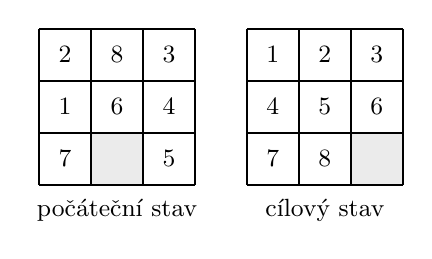
\begin{tikzpicture}[scale=0.66, every node/.style={font=\small}]
% počáteční stav: 2 8 3 / 1 6 4 / 7 _ 5  (volné pole sloupec 1, řádek 0)
\fill[black!8] (1,0) rectangle (2,1);
\draw[thick] (0,0) grid (3,3);
\foreach \c/\r/\v in {0/2/2,1/2/8,2/2/3, 0/1/1,1/1/6,2/1/4, 0/0/7,2/0/5}
  {\node at (\c+0.5,\r+0.5) {\v};}
\node at (1.5,-0.5) {počáteční stav};
% cílový stav: 1 2 3 / 4 5 6 / 7 8 _  (volné pole sloupec 2, řádek 0)
\begin{scope}[shift={(4,0)}]
\fill[black!8] (2,0) rectangle (3,1);
\draw[thick] (0,0) grid (3,3);
\foreach \c/\r/\v in {0/2/1,1/2/2,2/2/3, 0/1/4,1/1/5,2/1/6, 0/0/7,1/0/8}
  {\node at (\c+0.5,\r+0.5) {\v};}
\node at (1.5,-0.5) {cílový stav};
\end{scope}
\end{tikzpicture}
\obrpopis{8-puzzle: počáteční stav $\big[\begin{smallmatrix}2&8&3\\1&6&4\\7&\cdot&5\end{smallmatrix}\big]$ a~cílový stav $\big[\begin{smallmatrix}1&2&3\\4&5&6\\7&8&\cdot\end{smallmatrix}\big]$ (tečka = volné pole). Hodnoty heuristik v~počátečním stavu: $h_1=6$ (špatně umístěné kostky $2,8,1,6,4,5$), $h_2=9$ (Manhattan, oba odhady přípustné i~konzistentní).}
\end{center}
\end{priklad}

\noindent V~\texttt{priklady/} je u~této otázky původní oříznutý obrázek z~PDF a~oficiální náčrt řešení.
